\begin{figure}[h]
	\centering
	%H=H1 U H2 U H3
	\begin{subfigure}[b]{.9\textwidth}
		\[H = H_{1} \union H_{2} \union H_{3}:
		\raisebox{-.5\height}
		{
			\begin{tikzpicture}
				\vertex (s) at (0,1) [label=left:$s$]{};
				\vertex (t) at (1,1) [label=right:$t$]{};
				\vertex (u) at (0,0) [label=left:$u$]{};
				\vertex (v) at (1,0) [label=right:$v$]{};
				\vertex (w) at (2,1) [label=below:$w$]{};
				\vertex (x) at (3,1) [label=below:$x$]{};
				\vertex (y) at (4,1) [label=below:$y$]{};
				\vertex (z) at (5,1) [label=below:$z$]{};
				\path
					(s) edge (t)
					(s) edge (u)
					(t) edge (v)
					(u) edge (v)
					(w) edge (x)
					(x) edge (y)
				;
			\end{tikzpicture}
		}\]
	\end{subfigure}
	
	%H1
	\begin{subfigure}[b]{.3\textwidth}
		\[H_{1}:
		\raisebox{-.5\height}
		{
			\begin{tikzpicture}
				\vertex (s) at (0,1) [label=left:$s$]{};
				\vertex (t) at (1,1) [label=right:$t$]{};
				\vertex (u) at (0,0) [label=left:$u$]{};
				\vertex (v) at (1,0) [label=right:$v$]{};
				\path
					(s) edge (t)
					(s) edge (u)
					(t) edge (v)
					(u) edge (v)
				;
			\end{tikzpicture}
		}\]
	\end{subfigure}%
	%H2
	\begin{subfigure}[b]{.3\textwidth}
		\[H_{2}:
		\raisebox{-.5\height}
		{
			\begin{tikzpicture}
				\vertex (w) at (0,1) [label=below:$w$]{};
				\vertex (x) at (1,1) [label=below:$x$]{};
				\vertex (y) at (2,1) [label=below:$y$]{};
				\path
					(w) edge (x)
					(x) edge (y)
				;
			\end{tikzpicture}
		}\]
	\end{subfigure}%
	%H3
	\begin{subfigure}[b]{.3\textwidth}
		\[H_{3}:
		\raisebox{-.5\height}
		{
			\begin{tikzpicture}
				\vertex (z) at (0,1) [label=below:$z$]{};
			\end{tikzpicture}
		}\]
	\end{subfigure}
	\caption{A disconnected graph and its components}
\end{figure}